\chapter{Metodología}

\label{Chapter3}

En este capítulo se detallarán los procesos abordados para la extracción y clasificación de los dígitos escritos en los
telegramas de las elecciones. Primero se describirá el proceso de obtención, limpieza y transformación de los datos a
fin de obtener un conjunto de datos con el cual entrenar. Luego, se describirán los procesos a ser llevados a cabo para
el diseño experimental de los modelos.

\section{Descripción de los datos}

Los telegramas fueron descargados desde la \href{https://op.elecciones.gob.ar/telegramas/generales2021/}{página oficial
    del estado argentino} en formato TIFF. Los mismos presentan un formato estándar en forma de grilla, en la que se
encuentran los partidos políticos y los votos obtenidos para diputados y senadores en cada renglón. En la página
también se puede descargar un archivo en formato CSV donde se encuentra el identificador de cada telegrama y los
valores digitalizados oficialmente.

\section{Extracción de dígitos de los telegramas}

Durante las elecciones en Santa Fe, los telegramas de los votos presentaron un formato tabular en el que cada fila
representaba a un partido político y los votos obtenidos se encontraban divididos por senadores y diputados. Para poder
utilizar estos datos y entrenar modelos de aprendizaje automático, fue necesario llevar a cabo un proceso de
extracción, transformación y carga (ETL) de los mismos.

Este proceso de ETL implicó la ejecución de múltiples pasos para extraer la información relevante de los telegramas y
transformarla en un formato adecuado para su uso en modelos de aprendizaje automático. En primer lugar, se utilizó la
librería OpenCV \parencite{opencv_library} para manipular las imágenes de los telegramas y poder llevar a cabo el proceso de ETL.

A continuación, se realizó la extracción de la información tabular de los telegramas, identificando las filas
correspondientes a cada partido político y los votos obtenidos por senadores y diputados. Este proceso también incluyó
la limpieza y validación de los datos para asegurar su calidad y confiabilidad.

Posteriormente, se transformaron los datos extraídos en un formato adecuado para su uso en modelos de aprendizaje
automático. Esto implicó la normalización de los datos, la codificación de variables categóricas y la creación de
variables adicionales para mejorar la calidad de los datos. Finalmente, se cargó el conjunto de datos procesados en un
conjunto de datos que fue utilizado para entrenar los modelos.

\subsection{Alineación de los telegramas}
Cuando se escanean telegramas a mano, es común que estos no estén perfectamente alineados y presenten una ligera
inclinación en su posición. Por lo tanto, el primer paso en el procesamiento de los telegramas es alinearlos para
facilitar su lectura y análisis. Para lograr esto, se emplea un algoritmo que busca el rectángulo de mayor área en la
imagen del telegrama. Este rectángulo representa la región que abarca todo el contenido del telegrama y se utiliza para
calcular el ángulo de rotación necesario para alinear la imagen.

Una vez que se ha determinado el ángulo de rotación, se aplica una transformación geométrica a la imagen completa para
alinearla verticalmente. La misma se realiza calculando la siguiente matriz:

\begin{equation}
    \begin{bmatrix}
        \gamma & \beta  & (1-\gamma) \cdot  x - \beta \cdot y \\
        -\beta & \gamma & \beta \cdot  x - (1-\gamma) \cdot y \\
    \end{bmatrix}
    \label{eq:matriz-alineacion}
\end{equation}

\noindent
donde $\alpha$ es el ángulo de rotación de la imagen, $(x, y)$ es el centro de la imagen, $\gamma = \cos \alpha$ y $\beta = \sin \alpha$.
La figura \ref{fig:etl-1-rotacion} muestra un ejemplo del resultado que se obtiene al alinear los telegramas
de esta manera.

\begin{figure}[H]
    \centering

    \tikzset{every picture/.style={line width=0.75pt}}

    \begin{tikzpicture}[x=0.75pt,y=0.75pt,yscale=-1,xscale=1]

        \draw (370,140) node  {\frame{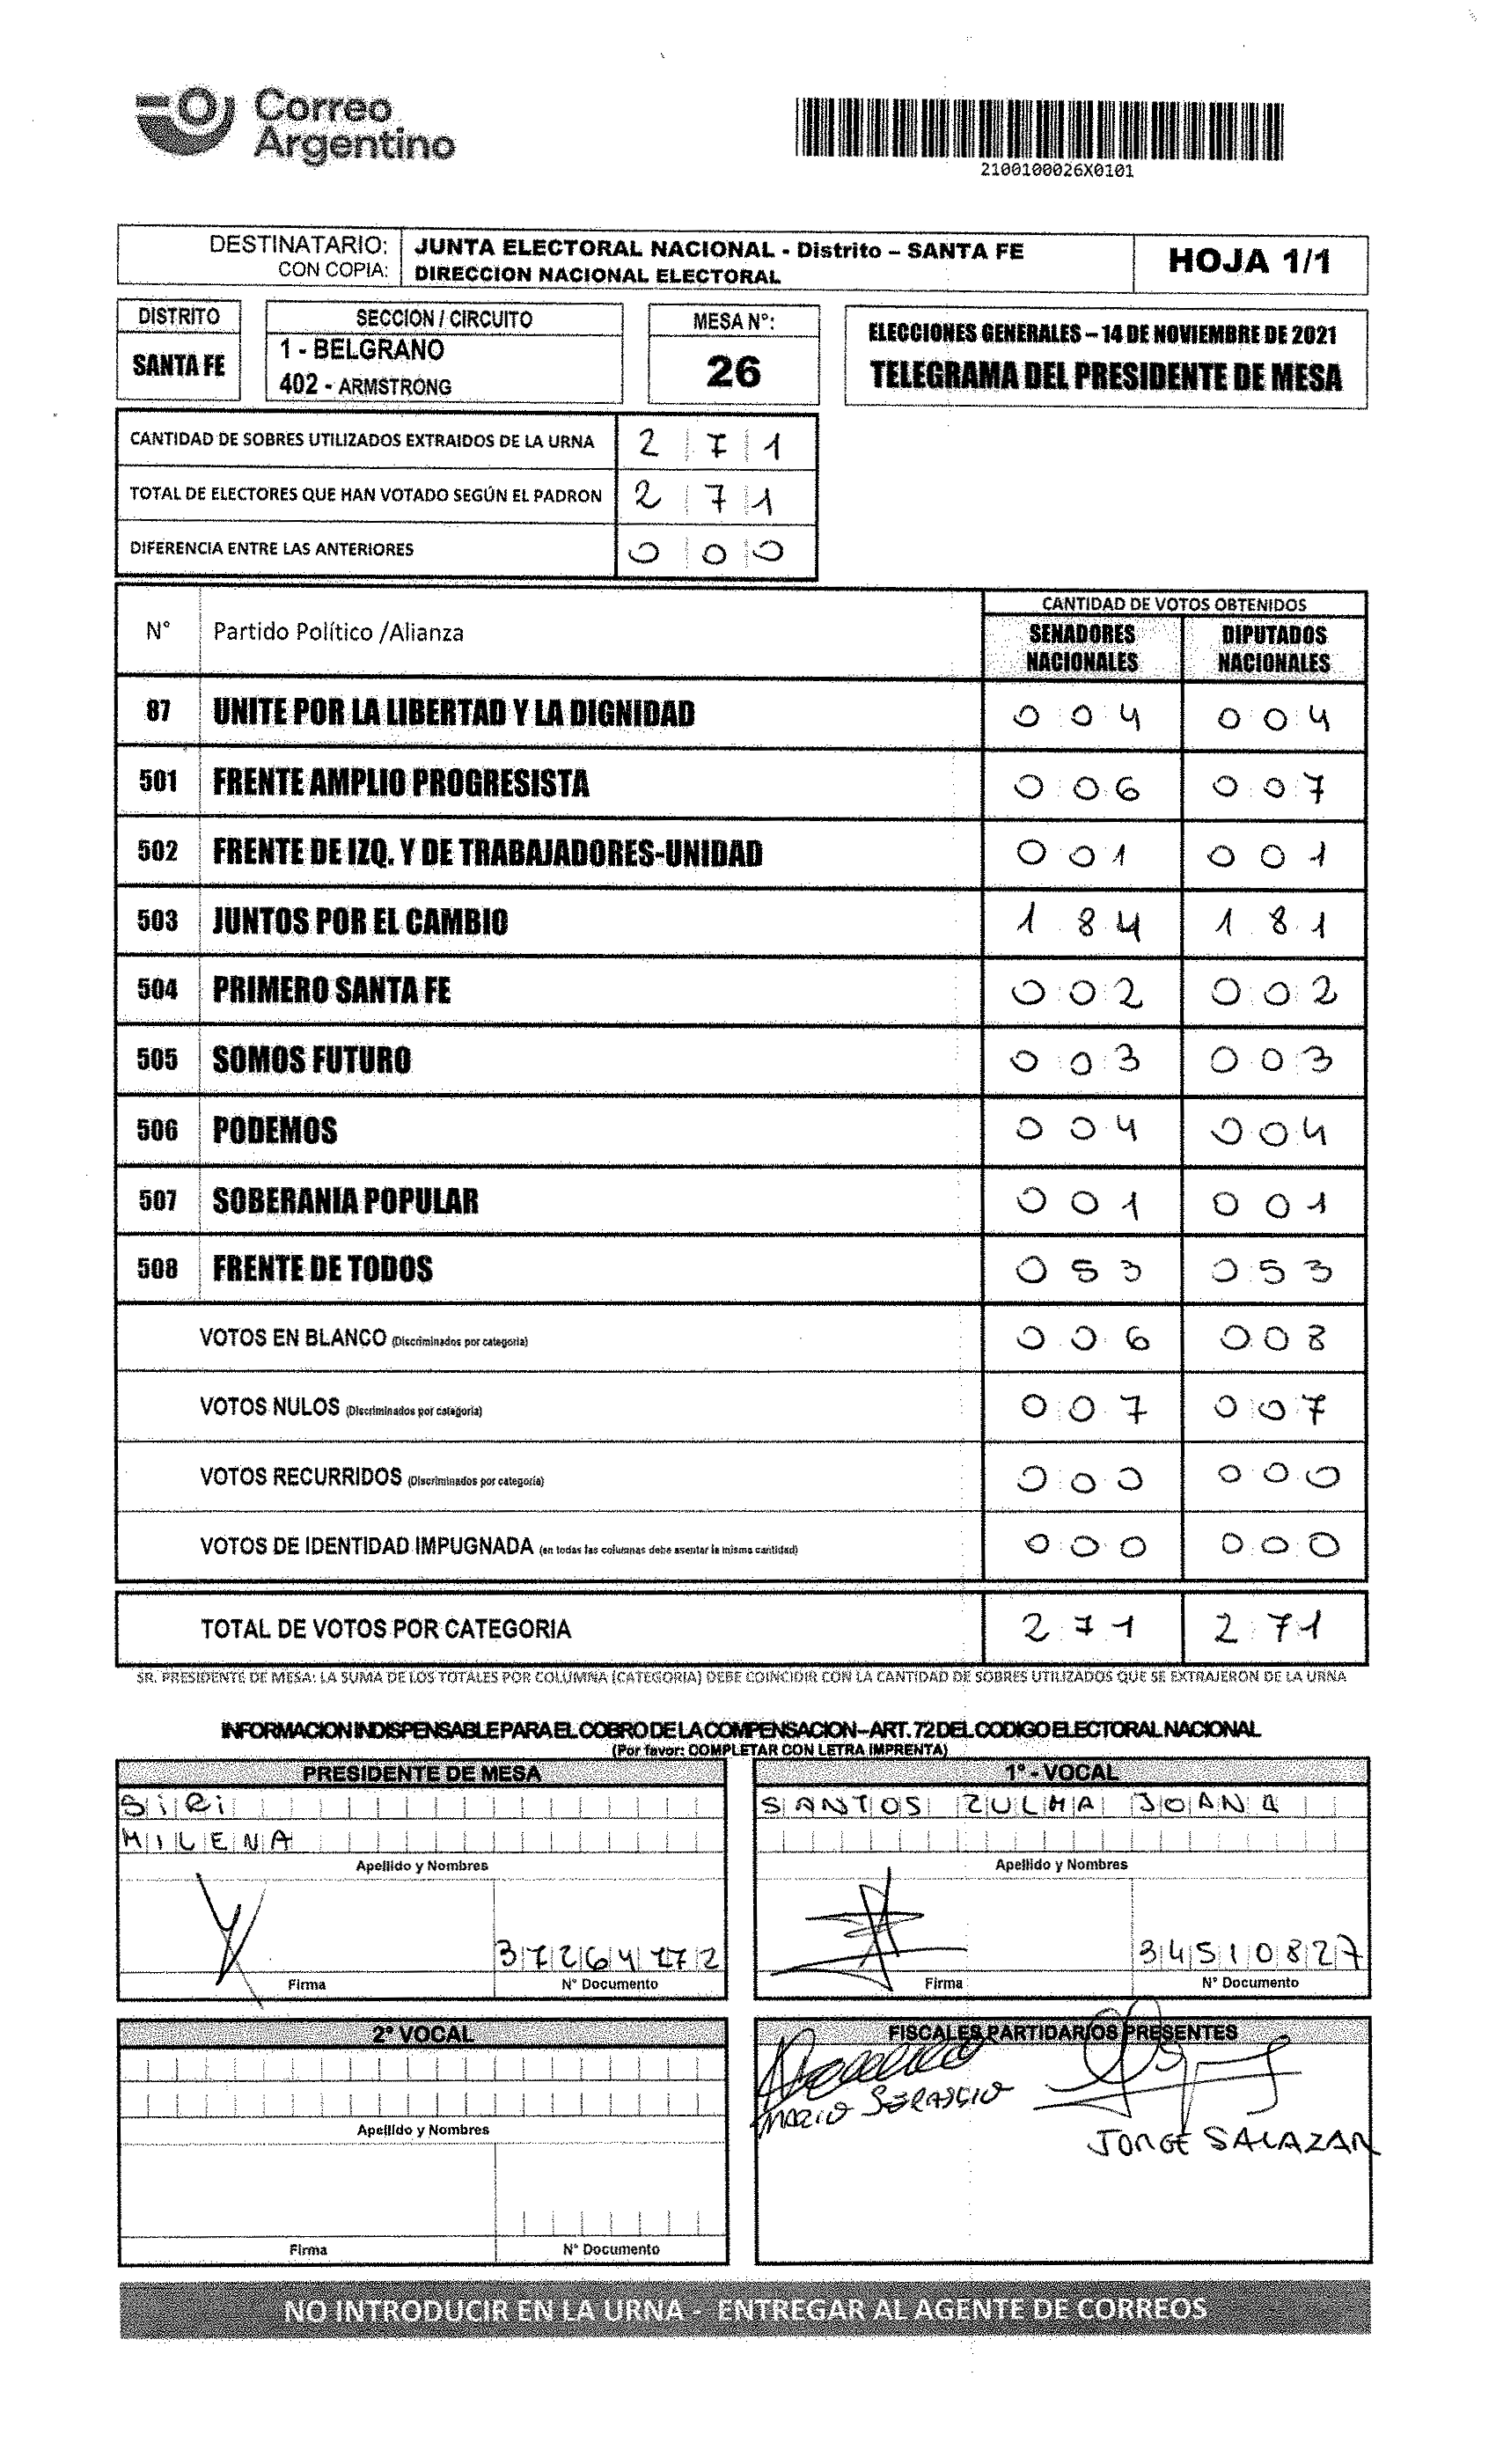
\includegraphics[width=135pt,height=210pt]{chapter3/etl-1-rotacion.png}}};
        \draw (90,140) node  {\frame{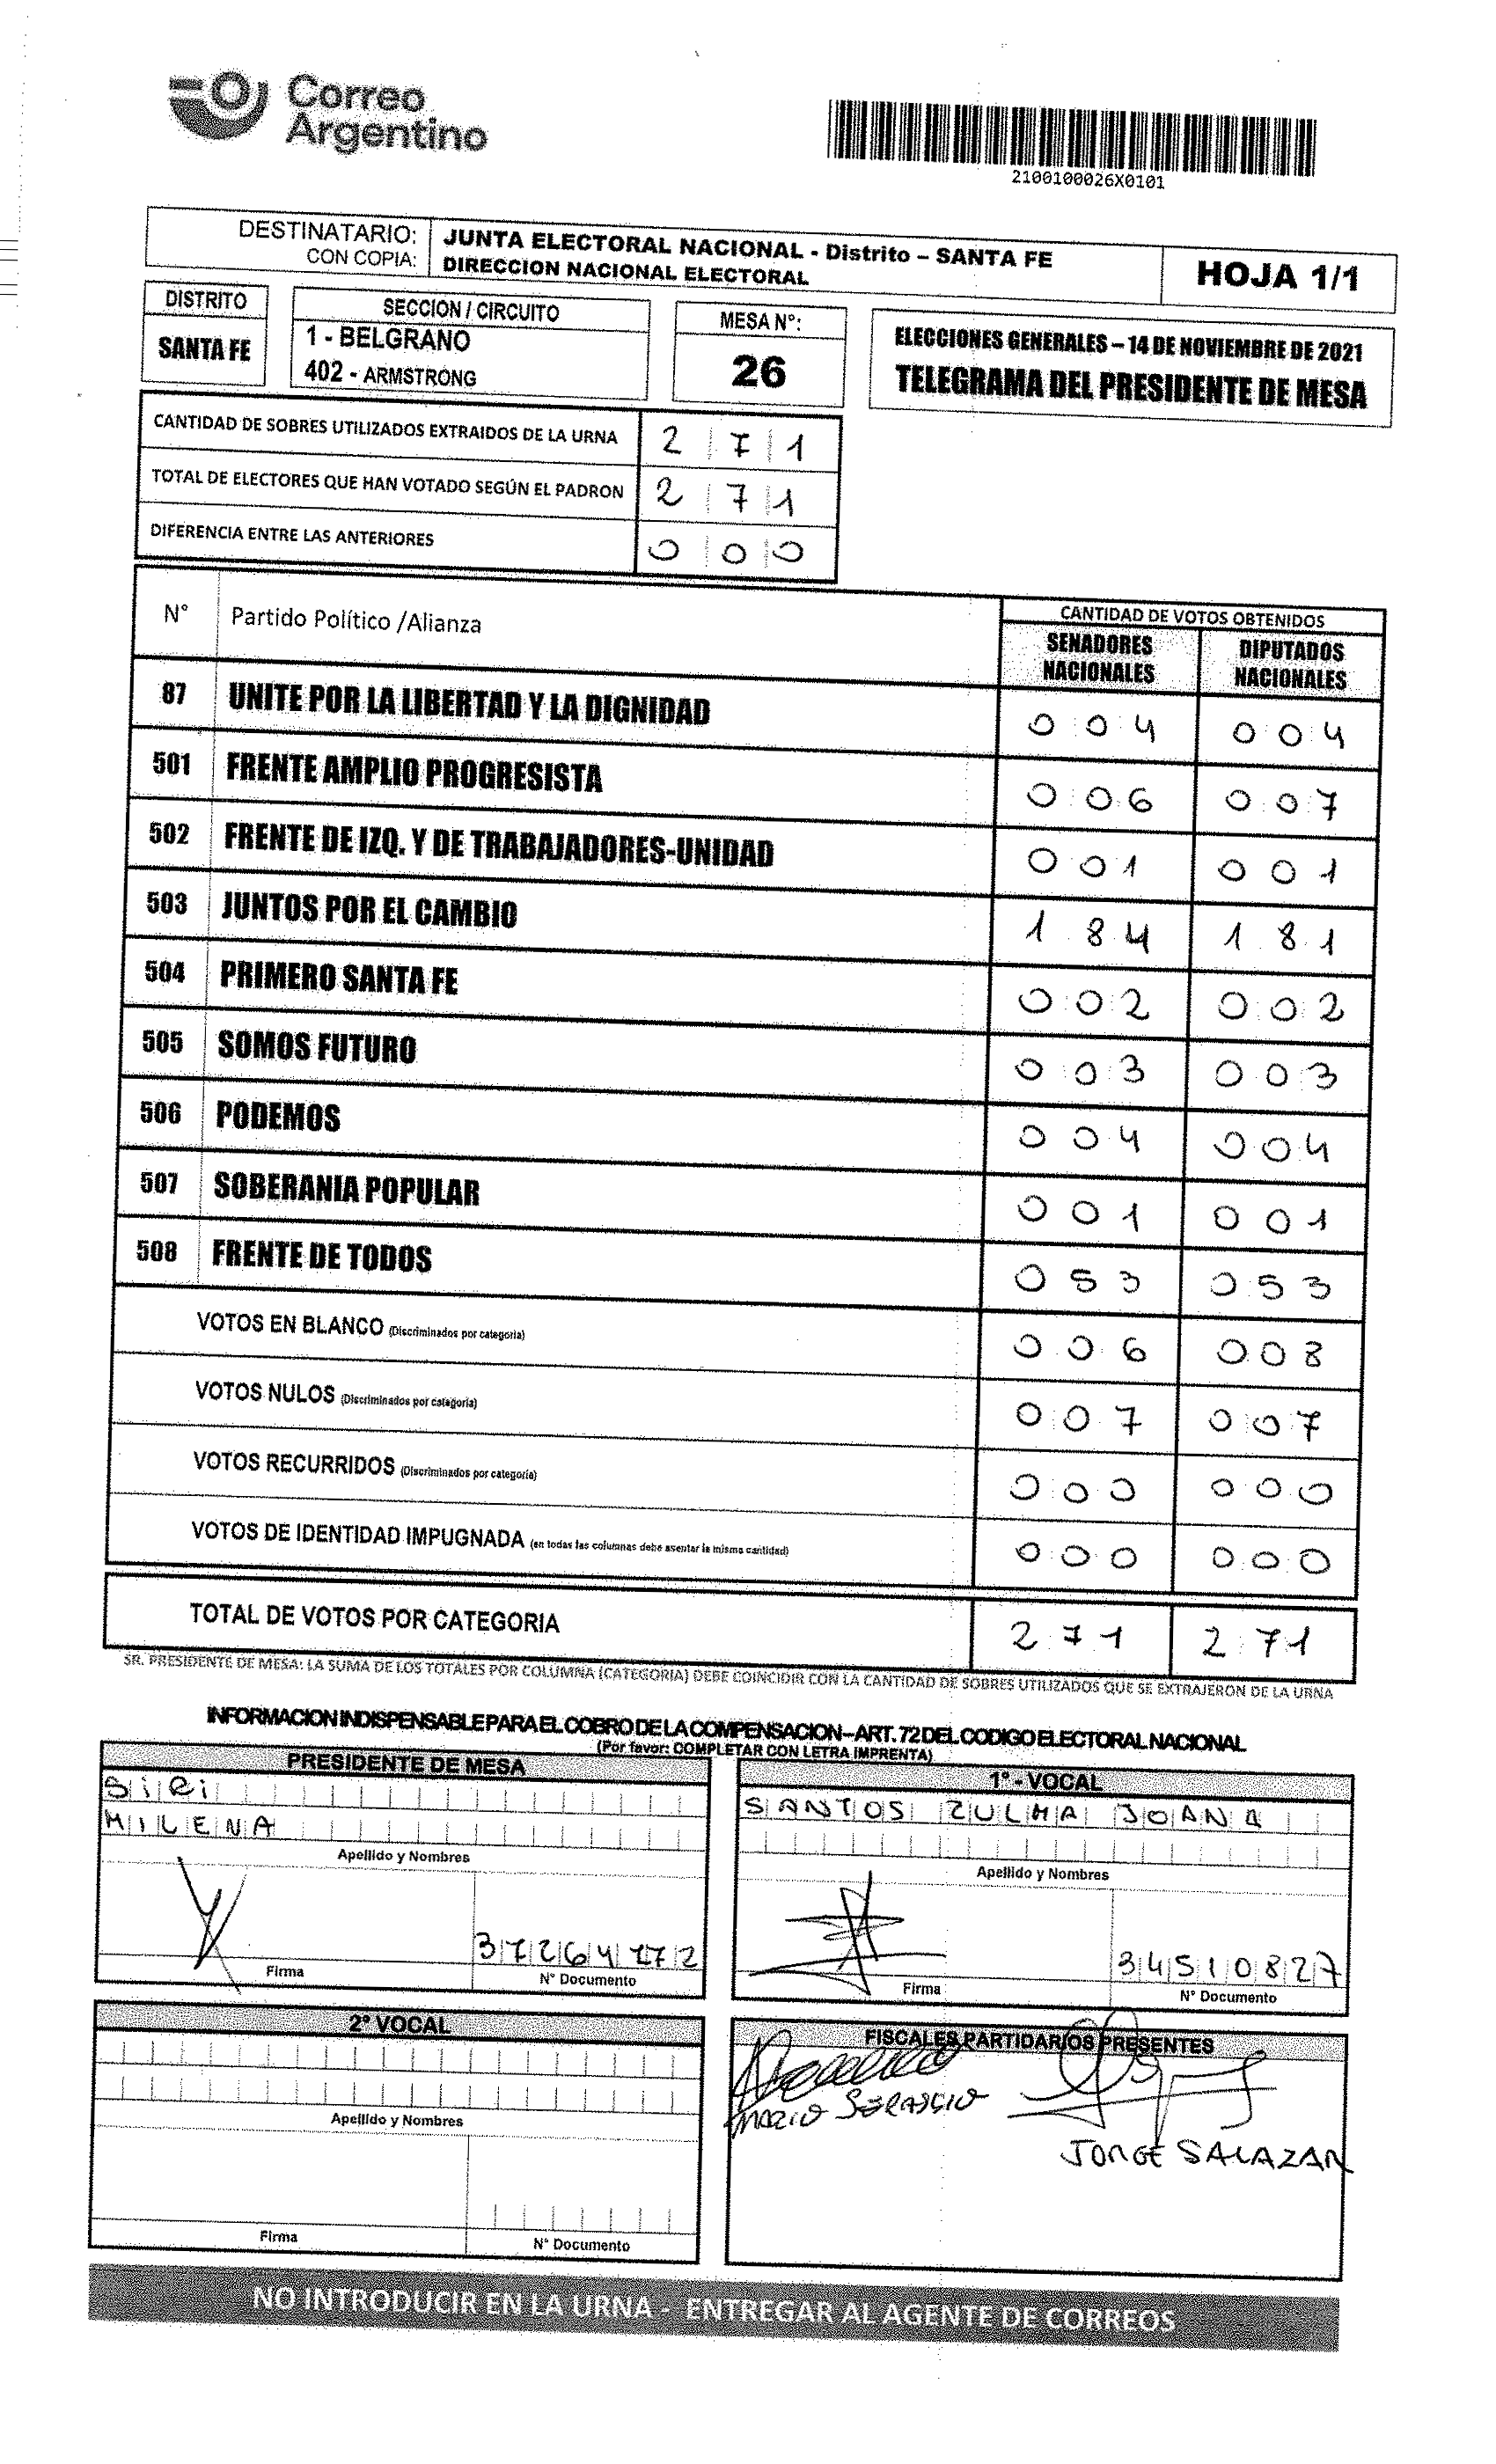
\includegraphics[width=135pt,height=210pt]{chapter3/etl-1-telegrama.png}}};
        \draw    (190.8,110.6) -- (267.4,110.6) ;
        \draw [shift={(269.4,110.6)}, rotate = 180] [color={rgb, 255:red, 0; green, 0; blue, 0 }  ][line width=0.75]    (10.93,-3.29) .. controls (6.95,-1.4) and (3.31,-0.3) .. (0,0) .. controls (3.31,0.3) and (6.95,1.4) .. (10.93,3.29)   ;
        \draw (200,87.18) node [anchor=north west][inner sep=0.75pt]   [align=left] {Alinear};

    \end{tikzpicture}

    \caption[Alineación de un telegrama]{Proceso de alineación de un telegrama mediante el uso de OpenCV.}
    \label{fig:etl-1-rotacion}
\end{figure}

\subsection{Extracción de la grilla de votos}

El siguiente paso consiste en extraer la grilla de votos para trabajar con ella de manera aislada. Para lograrlo, se
aplicó el algoritmo de detección de contornos propuesto por \cite{suzuki1985topological}, el cual permite identificar y
seleccionar los contornos presentes en la imagen, correspondientes a los bordes que delimitan los objetos en ella.
Mediante la selección del contorno de mayor área, se obtiene la grilla de votos como un objeto independiente.
Posteriormente, se procede a extraer la grilla de votos y trabajar con ella de manera separada del resto de la imagen.
Esto simplifica el procesamiento de los datos y facilita la extracción y análisis de los votos presentes en la grilla.
La figura \ref{fig:etl-2-grilla} muestra la grilla extraída mediante este proceso.

\begin{figure}[H]
    \centering
    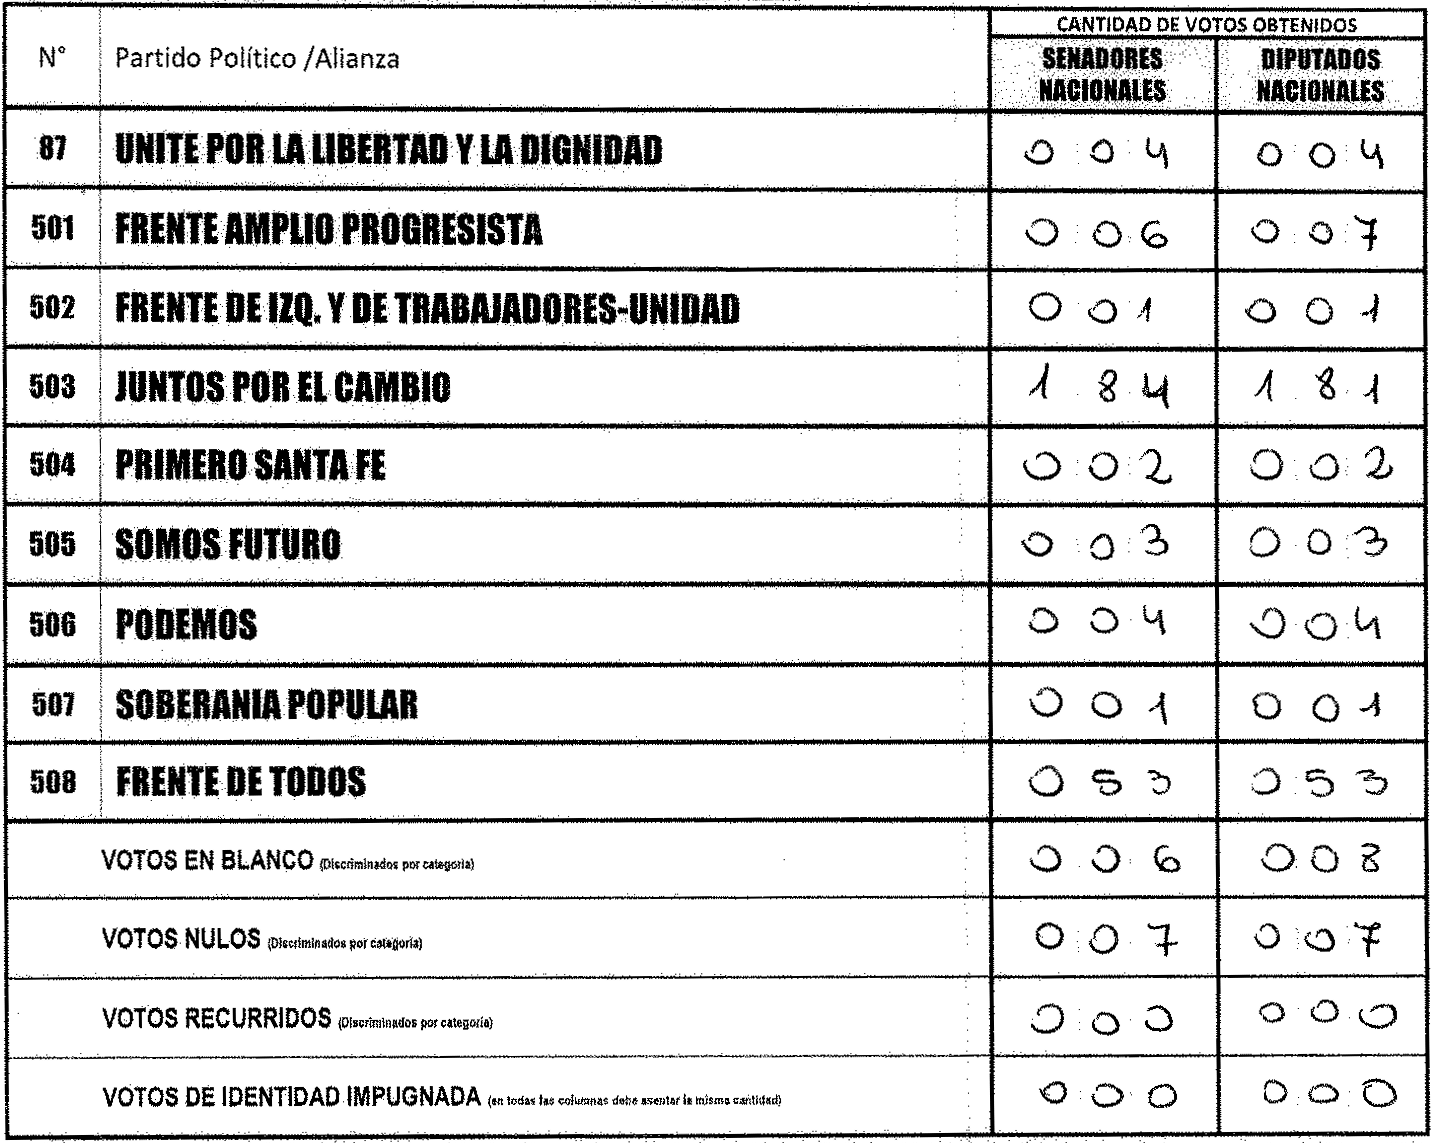
\includegraphics[width=0.4\textwidth, height=0.3\textwidth]{chapter3/etl-2-grilla.png}
    \caption[Grilla de votos detectada]{Grilla de votos extraída buscando el contorno de mayor área.}
    \label{fig:etl-2-grilla}
\end{figure}

\subsection{Detección de líneas de la grilla de votos}
Teniendo la grilla de votos separada del telegrama, se procede a detectar las líneas para poder extraer cada registro
de la misma. Se optó por utilizar un enfoque simplificado para la detección de líneas similar al utilizado en \parencite{lamagna2016lectura}. Debido a que la grilla se encuentra alineada verticalmente, se pueden utilizar las
proyecciones de los colores sobre los ejes $x$ e $y$ para detectarlas. Al sumar todos los colores por eje, se pueden
observar picos de valores donde se encuentran las líneas horizontales y verticales. Posteriormente, se selecciona un
umbral de corte por cada eje, siendo el mismo el promedio de cada eje menos dos desvíos estándar. La figura
\ref{fig:etl-3-proyecciones} muestra las proyecciones obtenidas con los umbrales por cada eje.

\begin{figure}[H]
    \centering

    \tikzset{every picture/.style={line width=0.75pt}}

    \begin{tikzpicture}[x=0.75pt,y=0.75pt,yscale=-1,xscale=1]
        \draw (142.77,162.65) node  {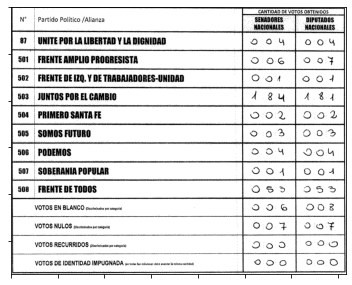
\includegraphics[width=214.16pt,height=173.4pt]{chapter3/etl-3-grilla.png}};
        \draw (303.6,159.11) node [rotate=-90] {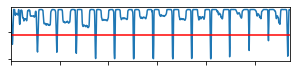
\includegraphics[width=172pt,height=46.15pt]{chapter3/etl-3-grilla-proyeccion-y.png}};
        \draw (142.5,30.77) node  {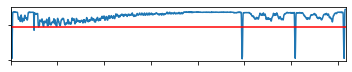
\includegraphics[width=213.75pt,height=46.15pt]{chapter3/etl-3-grilla-proyeccion-x.png}};
    \end{tikzpicture}

    \caption[Proyecciones de los ejes de la grilla de votos]{Proyecciones de los ejes de la grilla de votos. En rojo se marca el umbral de corte.}
    \label{fig:etl-3-proyecciones}
\end{figure}

Sin embargo, aunque se seleccionen aquellos píxeles que se encuentren por debajo del umbral, existe más de un píxel por
cada pico. Siguiendo con el ejemplo, en el eje $x$ se obtienen los siguientes píxeles que se encuentran en los
``picos'':

\begin{verbatim}
    array([    3,    4,    5,    6,    7,  100,  119,  120,  988, 
             989,  990,  991,  992, 1215, 1216, 1217, 1218, 1219, 
            1423, 1424, 1425, 1426, 1427])
\end{verbatim}

Con la estrategia del umbral no se obtienen las 4 líneas que se desean detectar sobre el eje $x$. No obstante, se puede
aplicar un clustering jerárquico sobre los índices obtenidos y luego calcular el índice promedio de cada clúster para
tomarlo como único representante. El proceso se repite de la misma manera sobre el eje $y$. Esta última modificación
sobre el trabajo realizado en \parencite{lamagna2016lectura} asegura tener un único píxel por línea. La figura \ref{fig:etl-3-grilla-detectada} muestra
la segmentación detectada mediante el proceso descrito.

\begin{figure}[H]
    \centering
    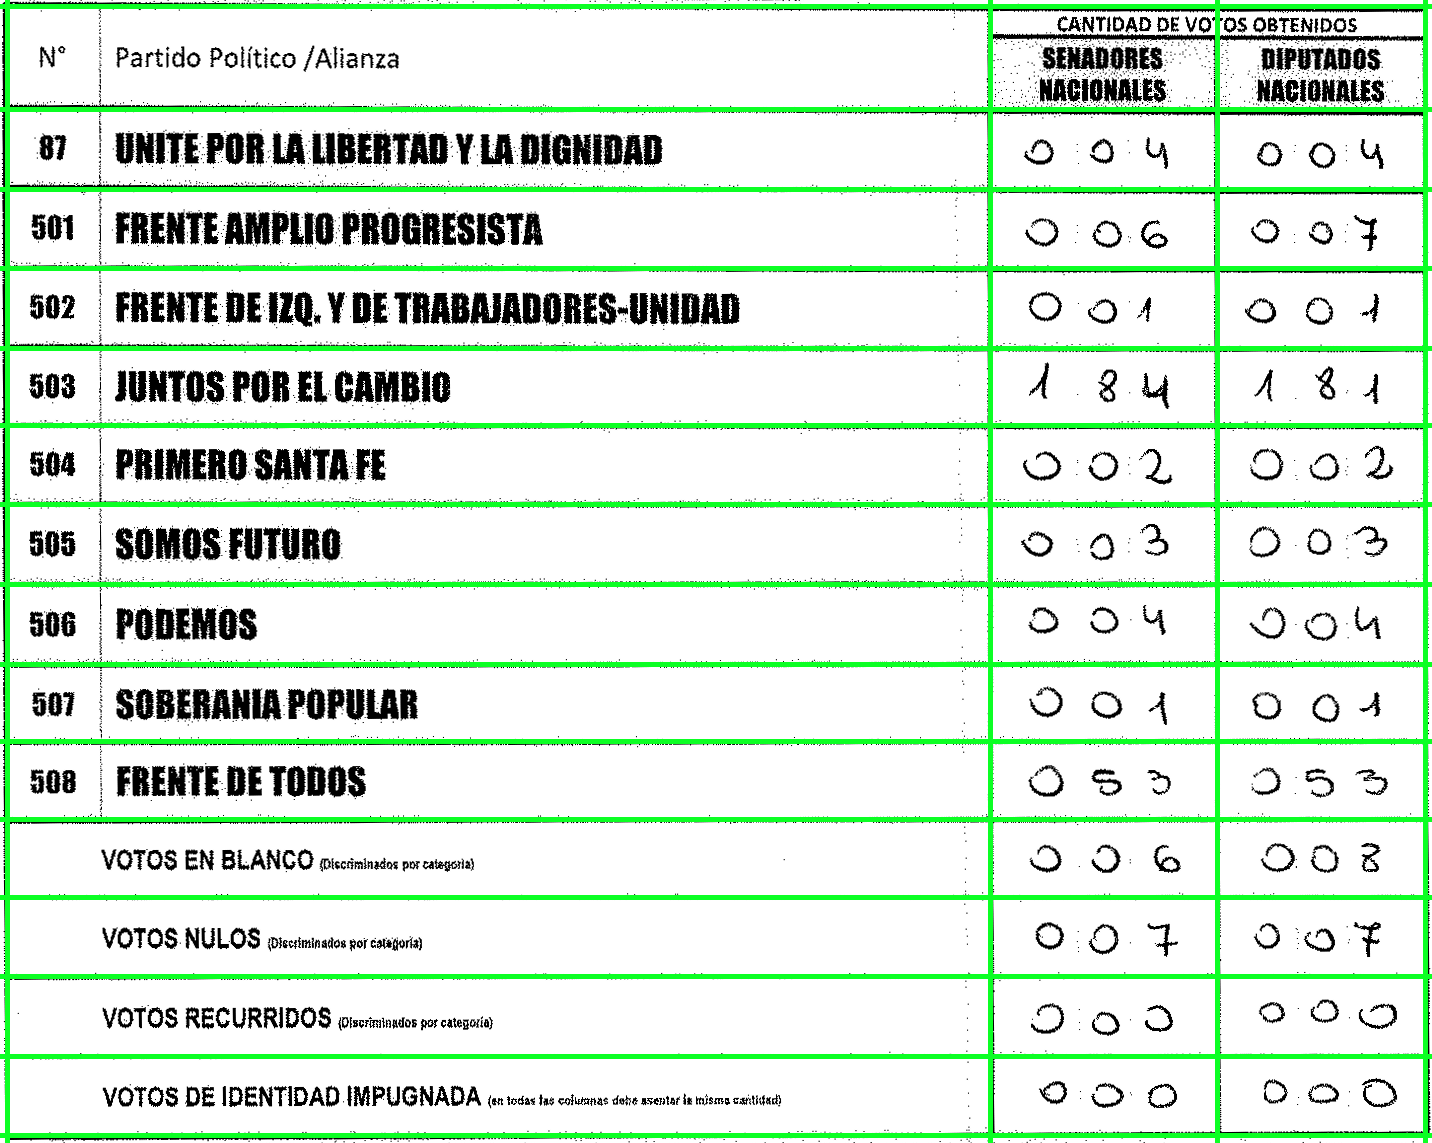
\includegraphics[width=0.4\textwidth, height=0.3\textwidth]{chapter3/etl-3-grilla-detectada.png}
    \caption[Segmentación de la grilla detectada]{Grilla detectada (en verde) utilizando el umbral por sobre las proyecciones y su posterior agrupamiento con clustering jerárquico.}
    \label{fig:etl-3-grilla-detectada}
\end{figure}

\subsection{Segmentación de dígitos}

Una vez obtenida la grilla, se itera por cada registro obteniendo los rectángulos que contienen los votos, ignorando el
primer renglón que contiene los títulos de la grilla. La figura \ref{fig:etl-4-registro} muestra un registro de la
grilla obtenida.

\begin{figure}[H]
    \centering
    \frame{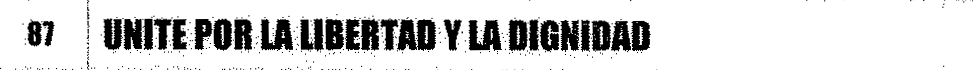
\includegraphics[height=15pt]{chapter3/etl-4-registro-1.png}}
    \frame{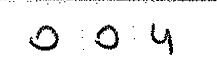
\includegraphics[height=15pt]{chapter3/etl-4-registro-2.png}}
    \frame{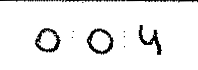
\includegraphics[height=15pt]{chapter3/etl-4-registro-3.png}}
    \caption[Primer registro extraído de la grilla de votos]{Primer registro extraído de la grilla de votos}
    \label{fig:etl-4-registro}
\end{figure}

Una vez obtenida la grilla de votos, se procede separar cada dígito de forma individual para poder procesarlos de forma
independiente. Para lograr esto, se utiliza un análisis de componentes conectados \parencite{bolelli2019spaghetti}, lo que permite identificar los distintos componentes (regiones conectadas) presentes en
una imagen binaria. En este caso, los componentes corresponden a los dígitos presentes en la grilla. Luego, se
establece un rango de áreas permitido para seleccionar los componentes que corresponden a los dígitos.

Para determinar el rango de áreas permitido, se realizó una experimentación previa y se establecieron como límites el
$5\%$ y el $70\%$ del total de píxeles de la imagen. De esta manera, se descartan aquellos contornos que representan
ruido o elementos no deseados que puedan haber sido detectados por el análisis de componentes conectados.

Una vez que se han identificado los componentes correspondientes a los dígitos, se procede a recortarlos
individualmente para obtener una imagen de cada dígito por separado. De esta manera, se facilita el procesamiento y
análisis de los votos de forma individual. La figura \ref{fig:etl-4-digitos} muestra los dígitos de un voto determinado
obtenidos de esta manera.

\begin{figure}[H]
    \centering
    \frame{
\includegraphics[scale=0.6]{chapter3/etl-4-digito-1.png}}
    \frame{
\includegraphics[scale=0.6]{chapter3/etl-4-digito-2.png}}
    \frame{
\includegraphics[scale=0.6]{chapter3/etl-4-digito-3.png}}
    \caption[Dígitos detectados en el primer bloque de votos]{Dígitos detectados en el primer bloque de votos}
    \label{fig:etl-4-digitos}
\end{figure}

Luego de haber realizado la segmentación de los dígitos, se procede a aplicar un proceso de transformación para que
todas las imágenes de dígitos tengan una dimensión cuadrada.

Finalmente, se lleva a cabo la construcción de un conjunto de datos que engloba información de los resultados
electorales. Este conjunto de datos se compone del partido político al que corresponde cada registro, lo cual se
determina a partir del orden de las filas en la tabla de votos. Además, se incluyen los dígitos correspondientes a los
votos emitidos y se registra el tipo de voto, ya sea senadores o diputados. Dicho proceso es realizado con el propósito
de poseer un conjunto de datos que posteriormente será utilizado para entrenar y validar los modelos.

\section{Análisis del conjunto de datos}

Una vez que se ha completado el proceso de extracción y segmentación de los dígitos, se procede a realizar un análisis
exploratorio de los datos. Este análisis tiene como objetivo detectar posibles errores o inconsistencias en los datos
extraídos, que puedan afectar la calidad de los modelos de aprendizaje automático que se construirán a partir de ellos.

La tabla \ref{tab:dataset-telegramas-segmentados} muestra algunos registros del conjunto de datos, que incluye
información como el número del telegrama, el partido político, el tipo de voto (senadores o diputados) y los dígitos
correspondientes a cada candidato.

\begin{table}[H]
    \centering
    \begin{tabular}{ccccc}
        \toprule
        Telegrama                                                               & Partido         & Tipo      & Dígitos                                                                  & \# Dígitos \\
        \midrule
        2100100026X                                                             & Unite           & Diputados & \frame{
\includegraphics[scale=0.6]{chapter3/eda/unite-diputados-1.png}}
        \frame{
\includegraphics[scale=0.6]{chapter3/eda/unite-diputados-2.png}}
        \frame{
\includegraphics[scale=0.6]{chapter3/eda/unite-diputados-3.png}} & 3                                                                                                                   \\
        2100100026X                                                             & Unite           & Senadores & \frame{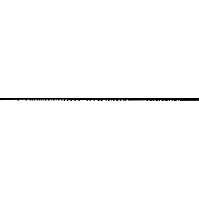
\includegraphics[scale=0.08]{chapter3/eda/unite-senadores-1.png}}
        \frame{
\includegraphics[scale=0.6]{chapter3/eda/unite-senadores-2.png}}
        \frame{
\includegraphics[scale=0.6]{chapter3/eda/unite-senadores-3.png}}
        \frame{
\includegraphics[scale=0.6]{chapter3/eda/unite-senadores-4.png}} & 4                                                                                                                   \\
        2100100067X                                                             & Frente de Todos & Diputados & \frame{
\includegraphics[scale=0.6]{chapter3/eda/todos-diputados-1.png}}
        \frame{
\includegraphics[scale=0.6]{chapter3/eda/todos-diputados-2.png}}
        \frame{
\includegraphics[scale=0.6]{chapter3/eda/todos-diputados-3.png}}
        \frame{
\includegraphics[scale=0.6]{chapter3/eda/todos-diputados-4.png}} & 4                                                                                                                   \\
        2100100067X                                                             & Frente de Todos & Senadores & \frame{
\includegraphics[scale=0.6]{chapter3/eda/todos-senadores-1.png}}
        \frame{
\includegraphics[scale=0.6]{chapter3/eda/todos-senadores-2.png}}
        \frame{
\includegraphics[scale=0.6]{chapter3/eda/todos-senadores-3.png}} & 3                                                                                                                   \\
        \bottomrule

    \end{tabular}
    \caption[Ejemplo del conjunto de datos generado]{Ejemplo de registros del conjunto de datos. Cada fila representa un voto.}
    \label{tab:dataset-telegramas-segmentados}
\end{table}

Se pueden detectar errores evidentes en la tabla presentada. En primer lugar, se puede observar que en la columna donde
solamente deben aparecer las imágenes de los dígitos, en el segundo registro existe una imagen de una línea horizontal,
lo cual no es correcto. Además, también se detectan dígitos mal escritos o enmendados, como los que se encuentran en
los dos últimos registros.

Para corregir estas extracciones incorrectas, se calculan dos columnas adicionales que contienen las proporciones
mínimas y máximas de píxeles blancos en las imágenes para cada voto. Estas proporciones permiten establecer un umbral
de confianza para las extracciones, de tal manera que aquellas imágenes con proporciones de píxeles blancos fuera de
los límites establecidos son descartadas.

Para visualizar de manera más clara la distribución de estas proporciones, se generan histogramas que muestran la
frecuencia de cada valor dentro del rango establecido. La figura \ref{fig:histogramas-min-max-prop-blanco} presenta
estos histogramas para las proporciones mínimas y máximas de píxeles blancos en las imágenes del conjunto de datos.

\begin{figure}[H]
    \centering
    \begin{subfigure}[h]{0.48\textwidth}
        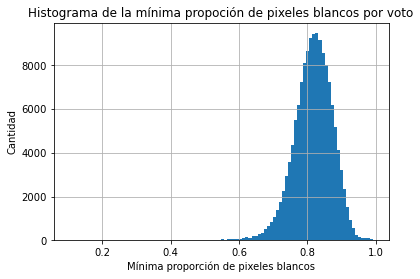
\includegraphics[width=1\textwidth]{chapter3/eda/hist-min-prop-blanco.png}
        \caption{Histograma de la proporción mínima de píxeles blancos en un voto.}
        \label{fig:histograma-min-prop-blanco}
    \end{subfigure}
    \hfill
    \begin{subfigure}[h]{0.48\textwidth}
        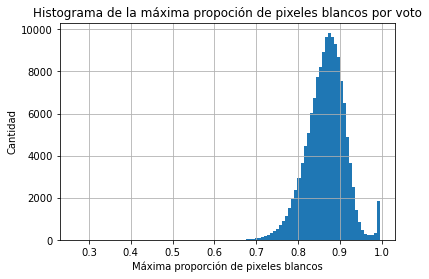
\includegraphics[width=1\textwidth]{chapter3/eda/hist-max-prop-blanco.png}
        \caption{Histograma de la proporción máxima de píxeles blancos en un voto.}
        \label{fig:histograma-max-prop-blanco}
    \end{subfigure}
    \caption[Histogramas de proporciones mínimas y máximas de píxeles blancos por voto]{Histogramas de proporciones de píxeles blancos por voto.}
    \label{fig:histogramas-min-max-prop-blanco}
\end{figure}

La cola derecha de la distribución de \ref{fig:histograma-max-prop-blanco} presenta un pico anormal en el extremo
cercano a 1. Al eliminar aquellas imágenes de dígitos que posean más de un $95\%$ de píxeles blancos, se logran
descartar los casos de líneas como la vista en el cuadro \ref{tab:dataset-telegramas-segmentados}. Por otro lado, al
eliminar aquellas imágenes que posean menos del $50\%$ de píxeles blancos, se logran descartar los casos de escritura
incorrecta.

El siguiente punto a analizar es el tamaño de las imágenes. Como se muestra en el cuadro
\ref{tab:dataset-telegramas-segmentados}, las imágenes no fueron estandarizadas en cuanto a tamaño. De manera análoga a
la variable de proporción de píxeles blancos, se calculan las variables de mínimo y máximo tamaño por voto. La tabla
\ref{tab:describe-min-max-size} muestra los estadísticos descriptivos de las mismas.

\begin{table}[H]
    \centering
    \begin{tabular}{crrrrr}
        \toprule
        Variable      & Promedio & Desvío & Mínimo & Mediana & Máximo \\
        \midrule
        Tamaño mínimo & 38.35    & 9.61   & 13     & 37      & 621    \\
        Tamaño máximo & 44.80    & 10.73  & 18     & 43      & 621    \\
        \bottomrule
    \end{tabular}
    \caption[Estadísticos descriptivos de los dígitos]{Estadísticos descriptivos del mínimo y máximo tamaño de las imágenes de los votos.}
    \label{tab:describe-min-max-size}
\end{table}

Al analizar aquellos registros que poseen los valores extremos en cuanto a mínimo y máximo de tamaño, se encuentran
telegramas que fueron cargados de forma incorrecta (ver anexo \ref{anexo:telegrama-erroneo}) o con una caligrafía en la
cual los dígitos no están separados entre sí, provocando que la segmentación por el análisis de componentes conectados
falle (ver anexo \ref{anexo:telegrama-numeros-juntos}). Se eliminan estos casos filtrando por aquellos registros que se
encuentren por fuera de la media más/menos cuatro desvíos estándar.

Una vez finalizada la etapa de análisis y limpieza, se exportan los dígitos extraídos en un formato similar al conocido
conjunto de datos {\it MNIST} junto con la etiqueta correspondiente. Este conjunto de datos será denominado {\it TDS}
(conjunto de datos de telegramas) a partir de este momento. El conjunto de datos {\it TDS} consta de un total de
170.718 imágenes de dígitos cuadradas con sus dimensiones originales, es decir, no se han estandarizado en una
dimensión específica. Esta decisión se tomó intencionalmente, ya que podría permitir una mayor flexibilidad en el
perfeccionamiento, procesamiento y análisis de los mismos en trabajos futuros. La figura \ref{fig:tds} muestra una
previsualización del conjunto de datos TDS.

\begin{figure}[H]
    \centering
    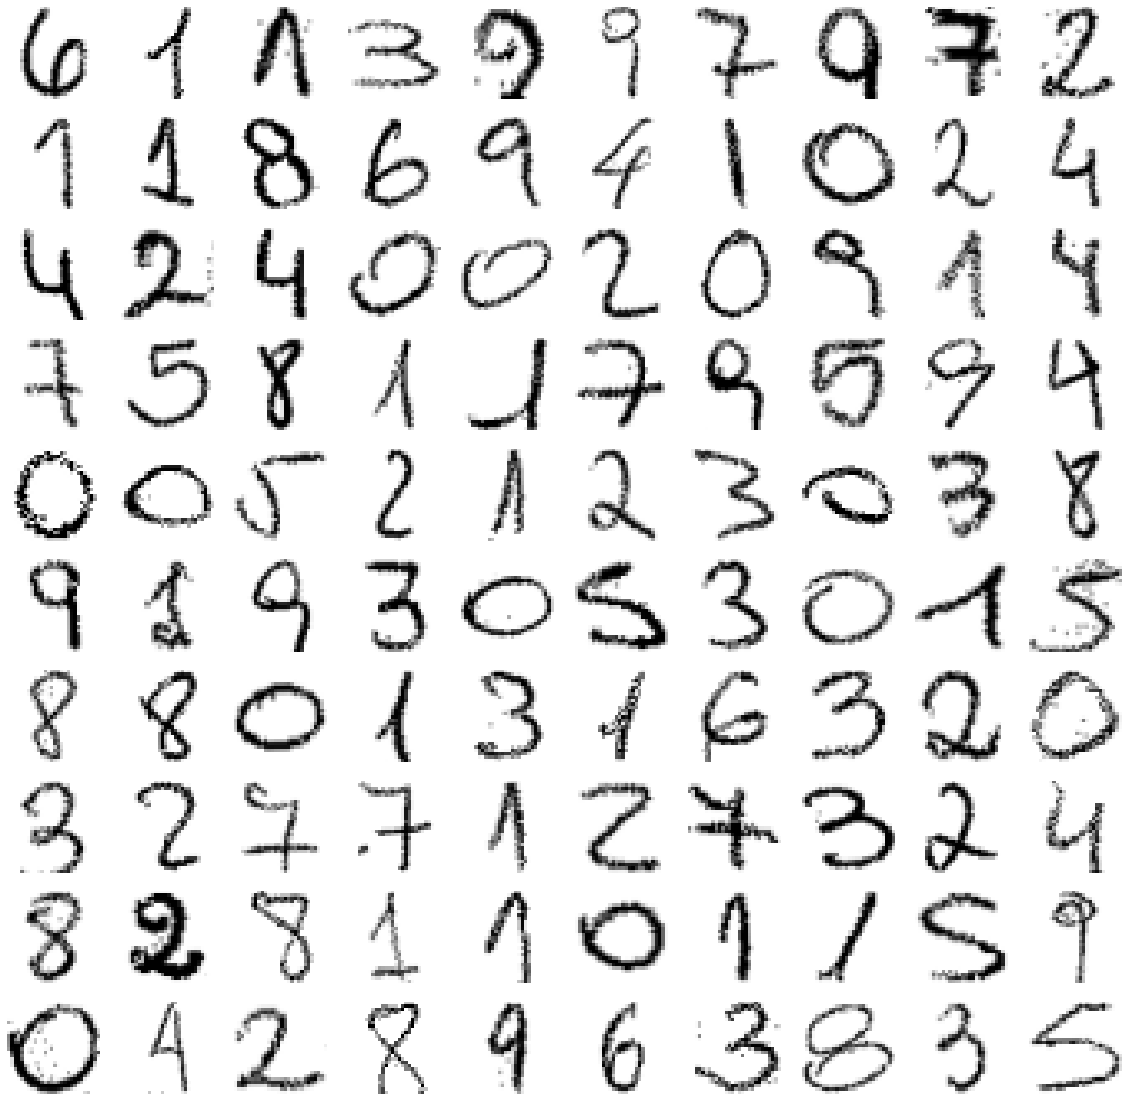
\includegraphics[width=0.5\textwidth]{chapter3/tds.png}
    \caption[Conjunto de datos TDS]{Muestra de 100 dígitos del conjunto de datos TDS}
    \label{fig:tds}
\end{figure}

\section{Diseño experimental}

Se llevaron a cabo experimentos con el fin de evaluar el desempeño de dos redes neuronales convolucionales, la ResNet18 \parencite{he2016deep} y la LeNet-8 \parencite{lecun1998gradient}, para cada una de las técnicas de adaptación de dominio que fueron descritas en el capítulo
\ref{Chapter2}. Además, como modelo de referencia, se entrenaron ambas redes sin ninguna técnica de adaptación. De esta
manera, se busca comparar el rendimiento de las redes con y sin técnicas de adaptación de dominio, para determinar cuál
técnica es la más adecuada para el problema en cuestión.

Las tecnologías utilizadas son:

\begin{itemize}
    \item Python como lenguaje de programación general.
    \item PyTorch \parencite{paszke2019pytorch} para la implementación de los modelos.
    \item PyTorch Lightning \parencite{falcon2019pytorch-lightning} para simplificar el entrenamiento de los modelos.
    \item TLLIB \parencite{tllib} para aplicar las técnicas de adaptación de dominio.
\end{itemize}

\subsection{Metodología de entrenamiento}

Para entrenar modelos mediante adaptación de dominio, se necesitan dos conjuntos de datos: uno etiquetado, llamado
origen, y otro sin etiquetar, llamado destino. En los experimentos llevados a cabo, se utilizó el conjunto de datos
    {\it MNIST} como origen y el conjunto de datos {\it TDS} como destino. Durante cada iteración de entrenamiento, se
proporcionó un lote de 1024 imágenes del conjunto de datos de origen y otro igual del conjunto de datos de destino. Se
realizaron tres particiones para cada conjunto de datos:

\begin{itemize}
    \item Entrenamiento (70\% de cada conjunto de datos): utilizado para entrenar la LeNet-8 y ResNet18 en cada época.
    \item Validación (15\% de cada conjunto de datos): utilizado para calcular los mejores hiperparámetros del modelo.
    \item Test (15\% de cada conjunto de datos): utilizado para calcular las métricas y gráficos finales del modelo entrenado.
\end{itemize}

Los modelos se entrenaron utilizando Stochastic Gradient Descent (SGD) \parencite{sutskever2013importance} utilizando nesterov, 0.9 como momento y 0.001 de weight decay, parámetros recomendados
para este tipo de aplicaciones.

\subsection{Selección y optimización del modelo}

La optimización de hiperparámetros se realizó utilizando la librería Optuna \parencite{optuna_2019}. Se ejecutaron 30 rondas de optimización con 10 épocas de entrenamiento por cada experimento. En
cada uno de los experimentos, se optimizaron los hiperparámetros para minimizar la función de pérdida de cada modelo.
El cuadro \ref{tab:rangos-hiperparametros} muestra los rangos de búsqueda para cada modelo, incluyendo el modelo de
referencia (sin adaptación de dominio).

\begin{table}[H]
    \centering
    \begin{tabular}{l|cccccc}
        \toprule
                   & {\it DANN}  & {\it ADDA}  & {\it DANN+BSP} & {\it MDD}   & {\it AFN}    & {\it Sin AD} \\
        \midrule
        $\eta_0$   & [1e-4, 0.1] & [1e-4, 0.1] & [1e-4, 0.1]    & [1e-4, 0.1] & [1e-4, 0.1]  & [1e-4, 0.1]  \\
        $\lambda$  & [0.5, 2]    & [0.5, 2]    & [0.5, 2]       & [0.5, 2]    & [0.001, 0.1] & -            \\
        $\beta$    & -           & -           & [1e-5, 0.1]    & -           & [0.0, 0.1]   & -            \\
        $\gamma$   & -           & -           & -              & [1, 10]     & -            & -            \\
        $\Delta_r$ & -           & -           & -              & -           & [0.01, 5]    & -            \\
        \# Blocks  & -           & -           & -              & -           & [1, 4]       & -            \\
        Dropout    & -           & -           & -              & -           & [0.3, 0.7]   & -            \\
        \bottomrule
    \end{tabular}
    \caption[Rango de hiperparámetros optimizados]{Rango de hiperparámetros optimizados para cada modelo.}
    \label{tab:rangos-hiperparametros}
\end{table}

Se implementó una disminución del learning rate en cada iteración de cada época, mediante la fórmula
\ref{eq:learning-rate}.

\begin{equation}
    \eta(t) = \eta_0 * (1 + \gamma_{\eta} * t)^{-\theta}
    \label{eq:learning-rate}
\end{equation}

\noindent
donde se optaron los valores de $\gamma_{\eta}=0.001$ y $\theta = 0.25$.

\section{Métricas de evaluación}

Los modelos optimizados serán evaluados con distintas métricas en tiempo de test, descritas en las siguientes
sub-secciones del capítulo. Las mismas pretenden evaluar qué tan buenos son los modelos respecto a la tarea de
clasificación y qué capacidad de adaptación de dominio poseen.

\subsection{Métricas de clasificación}
\subsubsection{Tasa de acierto}

La métrica de tasa de acierto (o {\it accuracy}) permite identificar qué tan cerca o lejos están los dígitos predichos
respecto a los de referencia. Es el ratio de predicciones correctas sobre las totales.

\begin{equation}
    Tasa \, de \, Acierto(y, \hat{y}) = \frac{1}{n} \sum_{i=0}^{n-1} 1(\hat{y_{i}}=y_{i})
\end{equation}

\noindent
donde:
\begin{itemize}
    \item $n$: es la cantidad de observaciones totales.
    \item $y_{i}$: es la clase de dígito de la ${i}$-ésima observación correspondiente al real.
    \item $\hat{y_{i}}$: es la clase de dígito predicho para la ${i}$-ésima observación.
    \item $1(x)$: es la función indicadora.
\end{itemize}

\subsubsection{$F_{1}$}

La métrica $F_{1}$ es una media armónica de otras dos: {\it precisión} y {\it sensibilidad}. De manera simplificada, la
primera muestra la capacidad del modelo de no etiquetar como positivo una observación que es negativa y la segunda
muestra la capacidad del modelo de encontrar todas las observaciones positivas.

La {\it sensibilidad} consiste en calcular la tasa de predicciones positivas correctas de la clase respecto al total de
predicciones positivas de la clase.

\begin{equation}
    Precision(y, \hat{y}) = \frac{TP}{TP + FP}
\end{equation}

\noindent
donde:
\begin{itemize}
    \item $TP$: es la cantidad de verdaderos positivos.
    \item $FP$: es la cantidad de falsos positivos.
\end{itemize}

Por otro lado, la {\it sensibilidad} consiste en calcular la tasa de predicciones positivas correctas de la clase
respecto al total de predicciones correctas de la clase.

\begin{equation}
    Sensibilidad(y, \hat{y}) = \frac{TP}{TP + FN}
\end{equation}

\noindent
donde:
\begin{itemize}
    \item $TP$: es la cantidad de verdaderos positivos.
    \item $FN$: es la cantidad de falsos negativos.
\end{itemize}

Las dos métricas mencionadas anteriormente pueden ser combinadas en una sola denominada $F_{\beta}$. El valor de
$\beta$ permite asignar un peso distinto a la precisión o a la sensibilidad dentro del promedio armónico. Cuando
$\beta=1$, ambas poseen el mismo peso.

\begin{equation}
    F_{\beta}(y, \hat{y}) = (1 + \beta^2) \times \frac{precision(y, \hat{y}) \times sensibilidad(y, \hat{y})}{\beta^2 \times precision(y, \hat{y}) + sensibilidad(y, \hat{y})}
\end{equation}

\noindent
El rango de valores es de $[0, 1]$, donde 1 corresponde a un clasificador que funciona sin errores.

\subsubsection{Intersección sobre unión}

Otra forma de evaluar al clasificador es mediante la {\it intersección sobre unión} (IoU por sus siglas en inglés).
Consta de calcular la cantidad de dígitos únicos predichos por sobre la cantidad de dígitos únicos reales. Por ejemplo,
para un telegrama y un partido el clasificador predice 189 votos cuando lo real es 180. Entonces, el {\it IoU} viene
dado por:

\begin{align}
    IoU(\{1, 8, 0\}, \{1, 8, 9\}) & = \frac{\lvert\{1, 8, 0\} \bigcap \{1, 8, 9\}\rvert}{\lvert\{1, 8, 0\} \bigcup \{1, 8, 9\}\rvert} \nonumber \\
                                  & = \frac{\lvert\{1, 8\}\rvert}{\lvert\{1, 8, 0, 9\}\rvert}                                         \nonumber \\
                                  & = \frac{2}{4}                                                                     \nonumber                 \\
                                  & = 0.5
\end{align}

\noindent
De forma general: sea $y_{i}$ el dígito $i$-ésimo del voto real $y$ de longitud $n$, $\hat{y_{j}}$ el dígito $j$-ésimo
del voto predicho por el modelo $\hat{y}$ de longitud $m$, entonces la métrica viene dada por:

\begin{equation}
    IoU(y, \hat{y}) = \frac{\lvert \{y_{i}\} \bigcap \{\hat{y_{j}}\}\rvert}{\lvert \{y_{i}\} \bigcup \{\hat{y_{j}}\}\rvert} \forall i \in \{1, \cdots, n\}, \forall j \in \{1, \cdots, m\}
\end{equation}

\subsection{Métricas de adaptación}
\subsubsection{Distancia $\mathcal{A}$}

La distancia $\mathcal{A}$ mide la similaridad entre dos distribuciones. Es muy utilizada para analizar los espacios
latentes de clasificadores en problemas de adaptación de dominio \parencite{ben2006analysis}. La métrica viene dada por:

\begin{equation}
    dist_\mathcal{A} = 2 (1-2\epsilon),
\end{equation}

\noindent
donde $\epsilon$ es el error en test de un clasificador entrenado para identificar el dominio de los ejemplos (origen o destino), por lo que su rango de valores es de cero al uno.
Cuando el error de clasificación es bajo, significa que hay diferencias significativas entre las dos distribuciones,
haciendo que $dist_\mathcal{A}$ sea grande y viceversa.

En la figura \ref{fig:ejemplos-dist-a} se muestran posibles casos de distribuciones de dominios. En la sub-figura
\ref{fig:dominios-distintos} las distribuciones de dominios son significativamente diferentes entre sí, por lo tanto
$dist_\mathcal{A} \approx 2$. Por el contrario, en la sub-figura \ref{fig:dominios-similares} las distribuciones de
dominios son similares entre sí, por lo que se espera que $dist_\mathcal{A} \approx 0$.

\begin{figure}[H]
    \centering
    \begin{subfigure}[h]{0.46\textwidth}
        \centering
        \tikzset{every picture/.style={line width=0.75pt}}
        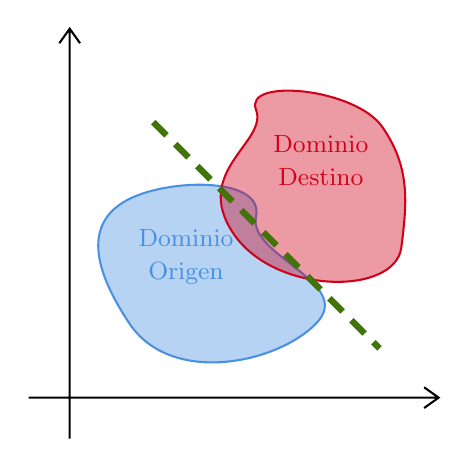
\begin{tikzpicture}[x=0.75pt,y=0.75pt,yscale=-1,xscale=1]
            \draw  (0,177.75) -- (197.5,177.75)(19.75,0) -- (19.75,197.5) (190.5,172.75) -- (197.5,177.75) -- (190.5,182.75) (14.75,7) -- (19.75,0) -- (24.75,7)  ;
            \draw  [color={rgb, 255:red, 74; green, 144; blue, 226 }  ,draw opacity=1 ][fill={rgb, 255:red, 74; green, 144; blue, 226 }  ,fill opacity=0.4 ] (48.5,82) .. controls (68.5,72) and (113.5,71.5) .. (109.5,90.5) .. controls (105.5,109.5) and (157.5,122.5) .. (138.5,142) .. controls (119.5,161.5) and (68.5,172) .. (48.5,142) .. controls (28.5,112) and (28.5,92) .. (48.5,82) -- cycle ;
            \draw  [color={rgb, 255:red, 208; green, 2; blue, 27 }  ,draw opacity=1 ][fill={rgb, 255:red, 208; green, 2; blue, 27 }  ,fill opacity=0.4 ] (109.5,39) .. controls (103.5,23.5) and (157.5,28.5) .. (170.5,47.5) .. controls (183.5,66.5) and (182.5,82.5) .. (179.5,105.5) .. controls (176.5,128.5) and (118.5,128.5) .. (98.5,98.5) .. controls (78.5,68.5) and (115.5,54.5) .. (109.5,39) -- cycle ;
            \draw (115,50) node [anchor=north west][inner sep=0.75pt]  [color={rgb, 255:red, 208; green, 2; blue, 27 }  ,opacity=1 ] [align=left] {\begin{minipage}[lt]{36.4pt}\setlength\topsep{0pt}
                    \begin{center}
                        {\small Dominio}\\{\small Destino}
                    \end{center}

                \end{minipage}};
            \draw (50,95) node [anchor=north west][inner sep=0.75pt]  [color={rgb, 255:red, 74; green, 144; blue, 226 }  ,opacity=1 ] [align=left] {\begin{minipage}[lt]{36.4pt}\setlength\topsep{0pt}
                    \begin{center}
                        {\small Dominio}\\{\small Origen}
                    \end{center}

                \end{minipage}};
            \draw [color={rgb, 255:red, 65; green, 117; blue, 5 }  ,draw opacity=1 ][line width=2.25]  [dash pattern={on 6.75pt off 4.5pt}]  (60,45) -- (169,154) ;
        \end{tikzpicture}
        \caption{Dominios distintos, discriminables.}
        \label{fig:dominios-distintos}
    \end{subfigure}
    \hfill
    \begin{subfigure}[h]{0.46\textwidth}
        \centering
        \tikzset{every picture/.style={line width=0.75pt}}

        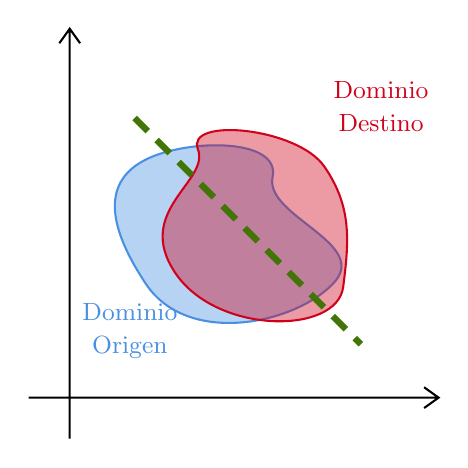
\begin{tikzpicture}[x=0.75pt,y=0.75pt,yscale=-1,xscale=1]
            \draw  (1,179.75) -- (198.5,179.75)(20.75,2) -- (20.75,199.5) (191.5,174.75) -- (198.5,179.75) -- (191.5,184.75) (15.75,9) -- (20.75,2) -- (25.75,9)  ;
            \draw  [color={rgb, 255:red, 74; green, 144; blue, 226 }  ,draw opacity=1 ][fill={rgb, 255:red, 74; green, 144; blue, 226 }  ,fill opacity=0.4 ] (57.5,65) .. controls (77.5,55) and (122.5,54.5) .. (118.5,73.5) .. controls (114.5,92.5) and (166.5,105.5) .. (147.5,125) .. controls (128.5,144.5) and (77.5,155) .. (57.5,125) .. controls (37.5,95) and (37.5,75) .. (57.5,65) -- cycle ;
            \draw  [color={rgb, 255:red, 208; green, 2; blue, 27 }  ,draw opacity=1 ][fill={rgb, 255:red, 208; green, 2; blue, 27 }  ,fill opacity=0.4 ] (82.5,60) .. controls (76.5,44.5) and (130.5,49.5) .. (143.5,68.5) .. controls (156.5,87.5) and (155.5,103.5) .. (152.5,126.5) .. controls (149.5,149.5) and (91.5,149.5) .. (71.5,119.5) .. controls (51.5,89.5) and (88.5,75.5) .. (82.5,60) -- cycle ;
            \draw [color={rgb, 255:red, 65; green, 117; blue, 5 }  ,draw opacity=1 ][line width=2.25]  [dash pattern={on 6.75pt off 4.5pt}]  (52,45) -- (161,154) ;

            \draw (24,133) node [anchor=north west][inner sep=0.75pt]  [color={rgb, 255:red, 74; green, 144; blue, 226 }  ,opacity=1 ] [align=left] {\begin{minipage}[lt]{36.4pt}\setlength\topsep{0pt}
                    \begin{center}
                        {\small Dominio}\\{\small Origen}
                    \end{center}

                \end{minipage}};
            \draw (145,26) node [anchor=north west][inner sep=0.75pt]  [color={rgb, 255:red, 208; green, 2; blue, 27 }  ,opacity=1 ] [align=left] {\begin{minipage}[lt]{36.4pt}\setlength\topsep{0pt}
                    \begin{center}
                        {\small Dominio}\\{\small Destino}
                    \end{center}

                \end{minipage}};
        \end{tikzpicture}

        \caption{Dominios similares, no discriminables.}
        \label{fig:dominios-similares}
    \end{subfigure}

    \caption[Ejemplos de distribuciones de dominios]{Ejemplos de distribuciones de dominios.}
    \label{fig:ejemplos-dist-a}
\end{figure}

Durante el proyecto se utiliza como clasificador una regresión logística a fin de calcular la distancia $\mathcal{A}$.

\subsubsection{Discrepancia de Medias Máxima}

La discrepancia de medias máxima (MMD por sus siglas en inglés) es una prueba estadística basada en {\it kernels} que
se utiliza para determinar si dos distribuciones dadas son iguales midiendo la distancia entre ellas \parencite{gretton2012kernel}. Dadas las distribuciones $P$ y $Q$ sobre un conjunto $\mathcal{X}$ y un mapa de
características $\phi : \mathcal{X} \rightarrow \mathcal{H}$ donde $\mathcal{H}$ es un conjunto de destino, MMD se
define como:

\begin{align}
    MMD^2(P, Q) = \left\lVert \mathbb{E}_{\mathbf{x} \sim P}[\phi(\mathbf{x})] - \mathbb{E}_{\mathbf{y} \sim Q}[\phi(\mathbf{y})]\right\rVert_{\mathcal{H}}^2
    \label{eq:mmd}
\end{align}

\noindent
Por ejemplo, si el mapa de características es $\phi(x)=x$ y $\mathcal{X}=\mathcal{H}=\mathbb{R}^d$, MMD se calcula
como:

\begin{align}
    MMD^2(P, Q) & = \left\lVert \mathbb{E}_{\mathbf{x} \sim P}[\phi(\mathbf{x})] - \mathbb{E}_{\mathbf{y} \sim Q}[\phi(\mathbf{y})] \right\rVert_{\mathcal{H}}^2 \nonumber \\
                & = \left\lVert \mathbb{E}_{\mathbf{x} \sim P}[\mathbf{x}] - \mathbb{E}_{\mathbf{y} \sim Q}[\mathbf{y}] \right\rVert_{\mathbb{R}^d}^2            \nonumber \\
                & = \left\lVert \mu_{P} - \mu_{Q} \right\rVert_{\mathbb{R}^d}^2,
    \label{eq:mmd-identidad}
\end{align}

\noindent
de forma que MMD es la distancia entre las medias de las distribuciones. No obstante, evaluarlas de esta manera puede
generar que distribuciones con distinta varianza, kurtosis, etc. sean consideradas como iguales. Se puede aplicar el
    {\it kernel trick} para calcular MMD con distancias más complejas. Dado $k(x, y) = \left\langle \phi(x), \phi(y)
    \right\rangle_{\mathcal{H}} $, MMD se calcula como:

\begin{align}
    MMD^2(P, Q) & = \left\lVert \mathbb{E}_{\mathbf{x} \sim P}[\phi(\mathbf{x})] - \mathbb{E}_{\mathbf{y} \sim Q}[\phi(\mathbf{y})] \right\rVert_{\mathcal{H}}^2 \nonumber                                                                          \\
                & = \mathbb{E}_{\mathbf{x}, \mathbf{x'} \sim P} k(\mathbf{x}, \mathbf{x'}) - \mathbb{E}_{\mathbf{y}, \mathbf{y'} \sim Q} k(\mathbf{y}, \mathbf{y'}) - 2 \mathbb{E}_{\mathbf{x} \sim P, \mathbf{y} \sim Q} k(\mathbf{x}, \mathbf{y})
    \label{eq:mmd-kernel}
\end{align}

\noindent
Se utilizó la librería TorchDrift \parencite{torchdrift} para implementarla en la evaluación de los modelos utilizando como {\it kernel} funciones de base
radial.